\documentclass[crop, tikz]{standalone}

\usetikzlibrary{math}
\begin{document}
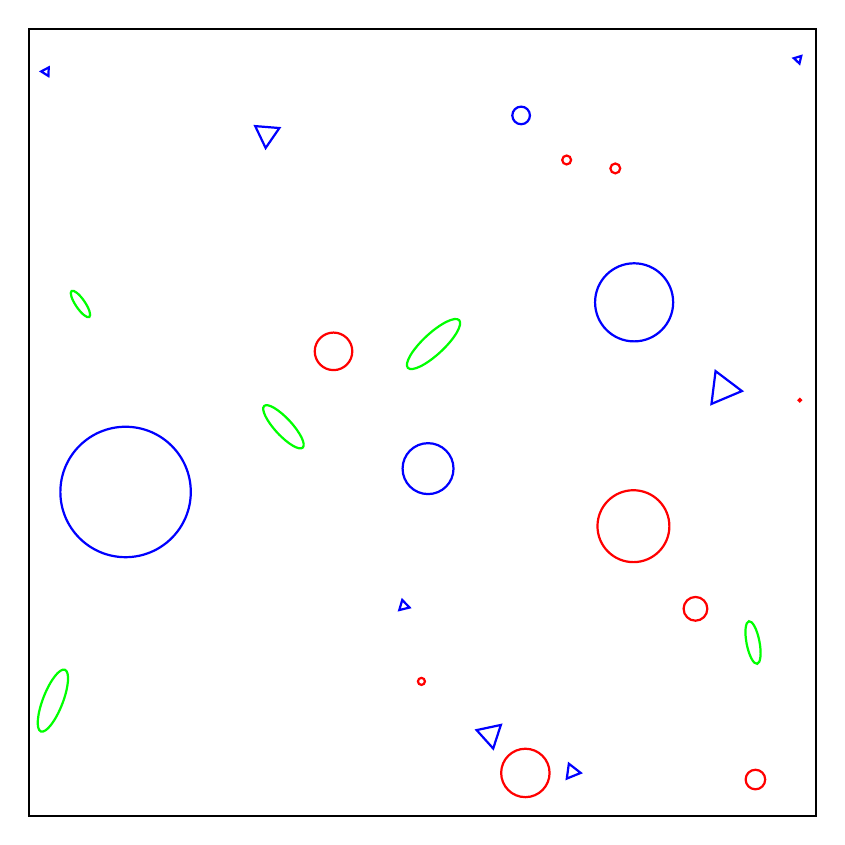
\begin{tikzpicture}
  \draw[thick] (0, 0) rectangle (10, 10);

  % red circles
  % import numpy as np
  % for x, y, r in zip(10*(np.random.random(5)), 10*(np.random.random(5)), 0.5*(np.random.random(5))):
  %     print(str(x)+'/'+str(y)+'/'+str(r)+',')

  \foreach \xcord / \ycord / \rcord in {
    7.679061860689958/3.682979874355471/0.4565838404947177,
    9.79222926473049/5.283254108481699/0.014712651759808348,
    9.228163854796406/0.465467574267856/0.12417262955376379,
    8.466903599867722/2.6335052370495404/0.15078170372073274,
    3.8702372331492265/5.903399027966185/0.23838775192054612,
    4.986562338321869/1.7117275570073676/0.044592439438311426,
    7.448863277700564/8.226461665494632/0.06244327990940718,
    6.306622283446704/0.5491178028038102/0.3074134849629631,
    6.831041908490814/8.333630001447492/0.05653784106297699
  }{
    \draw[red, thick] (\xcord, \ycord) circle (\rcord);
  }

  % blue circles
  \foreach \x / \y / \r in {
    1.2293473513913522/4.117458330953575/0.8282351326975819,
    7.687835189158383/6.525741647740903/0.4959151367782896,
    5.07067407779401/4.413937901291682/0.32343724210759717,
    6.252736357650197/8.899430585033288/0.11194328613448434
  }{
    \draw[blue, thick] (\x, \y) circle (\r);
  }

  % green ellipses
  \foreach \x / \y / \a / \b / \ang in {
    5.140384055187862/5.996278145733781/0.44458636535075624/0.13337590960522686/42.8959206218665,
    3.234418862988054/4.945278056645622/0.36019401697947695/0.10805820509384308/132.77692008629268,
    0.6563379428642213/6.504964785235348/0.19991550807517933/0.059974652422553794/124.22338658231189,
    9.197961905303377/2.205439358917957/0.27526797473586584/0.08258039242075975/100.8813649933555,
    0.3062812177004437/1.4677046604730348/0.42017352508362876/0.12605205752508863/68.71741736618897
  }{
    \draw[green, thick, rotate around={\ang:(\x,\y)}] (\x, \y) ellipse (\a cm and  \b cm);
  }

  % blue triangles
  % import numpy as np
  % for x, y, a, ang in zip(10*(np.random.random(5)), 10*(np.random.random(5)), 0.5*(np.random.random(5)), 180*(np.random.random(5))):
  %    print(str(x)+'/'+str(y)+'/'+str(a)+'/'+str(0.3*a)+'/'+str(ang)+',')

  \foreach \x / \y / \a / \b / \ang in {
    3.1825266671917642/8.739378860463935/0.3076868629010771/0.09230605887032313/55.44224580874666,
    5.9953999833826535/1.1586268023457924/0.31485139062877743/0.09445541718863322/71.98786362988174,
    9.810321336977507/9.65425711309965/0.09875441625998671/0.02962632487799601/76.7939584508893,
    9.05699195598717/5.39917055694529/0.419809206167695/0.1259427618503085/22.929429244839067,
    4.835379117540814/2.649414224653106/0.13385616813162254/0.04015685043948676/13.633175956536425,
    6.858701607071196/0.6665273841406083/0.19102094661889218/0.05730628398566765/142.1722416667769,
    0.25352036670998834/9.508868483290078/0.10883725448703785/0.03265117634611135/87.79022903558271
  }{
    \draw[blue, thick, rotate around={\ang:(\x,\y)}] (\x, \y) \foreach \s in {120, 240}{
      -- ++ (\s:\a)
    } -- cycle ++ (90:\a);
  }
\end{tikzpicture}
\end{document}
